% Options for packages loaded elsewhere
\PassOptionsToPackage{unicode}{hyperref}
\PassOptionsToPackage{hyphens}{url}
\PassOptionsToPackage{dvipsnames,svgnames,x11names}{xcolor}
%
\documentclass[
  letterpaper,
  DIV=11,
  numbers=noendperiod]{scrreprt}

\usepackage{amsmath,amssymb}
\usepackage{lmodern}
\usepackage{iftex}
\ifPDFTeX
  \usepackage[T1]{fontenc}
  \usepackage[utf8]{inputenc}
  \usepackage{textcomp} % provide euro and other symbols
\else % if luatex or xetex
  \usepackage{unicode-math}
  \defaultfontfeatures{Scale=MatchLowercase}
  \defaultfontfeatures[\rmfamily]{Ligatures=TeX,Scale=1}
\fi
% Use upquote if available, for straight quotes in verbatim environments
\IfFileExists{upquote.sty}{\usepackage{upquote}}{}
\IfFileExists{microtype.sty}{% use microtype if available
  \usepackage[]{microtype}
  \UseMicrotypeSet[protrusion]{basicmath} % disable protrusion for tt fonts
}{}
\makeatletter
\@ifundefined{KOMAClassName}{% if non-KOMA class
  \IfFileExists{parskip.sty}{%
    \usepackage{parskip}
  }{% else
    \setlength{\parindent}{0pt}
    \setlength{\parskip}{6pt plus 2pt minus 1pt}}
}{% if KOMA class
  \KOMAoptions{parskip=half}}
\makeatother
\usepackage{xcolor}
\setlength{\emergencystretch}{3em} % prevent overfull lines
\setcounter{secnumdepth}{5}
% Make \paragraph and \subparagraph free-standing
\ifx\paragraph\undefined\else
  \let\oldparagraph\paragraph
  \renewcommand{\paragraph}[1]{\oldparagraph{#1}\mbox{}}
\fi
\ifx\subparagraph\undefined\else
  \let\oldsubparagraph\subparagraph
  \renewcommand{\subparagraph}[1]{\oldsubparagraph{#1}\mbox{}}
\fi

\usepackage{color}
\usepackage{fancyvrb}
\newcommand{\VerbBar}{|}
\newcommand{\VERB}{\Verb[commandchars=\\\{\}]}
\DefineVerbatimEnvironment{Highlighting}{Verbatim}{commandchars=\\\{\}}
% Add ',fontsize=\small' for more characters per line
\usepackage{framed}
\definecolor{shadecolor}{RGB}{241,243,245}
\newenvironment{Shaded}{\begin{snugshade}}{\end{snugshade}}
\newcommand{\AlertTok}[1]{\textcolor[rgb]{0.68,0.00,0.00}{#1}}
\newcommand{\AnnotationTok}[1]{\textcolor[rgb]{0.37,0.37,0.37}{#1}}
\newcommand{\AttributeTok}[1]{\textcolor[rgb]{0.40,0.45,0.13}{#1}}
\newcommand{\BaseNTok}[1]{\textcolor[rgb]{0.68,0.00,0.00}{#1}}
\newcommand{\BuiltInTok}[1]{\textcolor[rgb]{0.00,0.23,0.31}{#1}}
\newcommand{\CharTok}[1]{\textcolor[rgb]{0.13,0.47,0.30}{#1}}
\newcommand{\CommentTok}[1]{\textcolor[rgb]{0.37,0.37,0.37}{#1}}
\newcommand{\CommentVarTok}[1]{\textcolor[rgb]{0.37,0.37,0.37}{\textit{#1}}}
\newcommand{\ConstantTok}[1]{\textcolor[rgb]{0.56,0.35,0.01}{#1}}
\newcommand{\ControlFlowTok}[1]{\textcolor[rgb]{0.00,0.23,0.31}{#1}}
\newcommand{\DataTypeTok}[1]{\textcolor[rgb]{0.68,0.00,0.00}{#1}}
\newcommand{\DecValTok}[1]{\textcolor[rgb]{0.68,0.00,0.00}{#1}}
\newcommand{\DocumentationTok}[1]{\textcolor[rgb]{0.37,0.37,0.37}{\textit{#1}}}
\newcommand{\ErrorTok}[1]{\textcolor[rgb]{0.68,0.00,0.00}{#1}}
\newcommand{\ExtensionTok}[1]{\textcolor[rgb]{0.00,0.23,0.31}{#1}}
\newcommand{\FloatTok}[1]{\textcolor[rgb]{0.68,0.00,0.00}{#1}}
\newcommand{\FunctionTok}[1]{\textcolor[rgb]{0.28,0.35,0.67}{#1}}
\newcommand{\ImportTok}[1]{\textcolor[rgb]{0.00,0.46,0.62}{#1}}
\newcommand{\InformationTok}[1]{\textcolor[rgb]{0.37,0.37,0.37}{#1}}
\newcommand{\KeywordTok}[1]{\textcolor[rgb]{0.00,0.23,0.31}{#1}}
\newcommand{\NormalTok}[1]{\textcolor[rgb]{0.00,0.23,0.31}{#1}}
\newcommand{\OperatorTok}[1]{\textcolor[rgb]{0.37,0.37,0.37}{#1}}
\newcommand{\OtherTok}[1]{\textcolor[rgb]{0.00,0.23,0.31}{#1}}
\newcommand{\PreprocessorTok}[1]{\textcolor[rgb]{0.68,0.00,0.00}{#1}}
\newcommand{\RegionMarkerTok}[1]{\textcolor[rgb]{0.00,0.23,0.31}{#1}}
\newcommand{\SpecialCharTok}[1]{\textcolor[rgb]{0.37,0.37,0.37}{#1}}
\newcommand{\SpecialStringTok}[1]{\textcolor[rgb]{0.13,0.47,0.30}{#1}}
\newcommand{\StringTok}[1]{\textcolor[rgb]{0.13,0.47,0.30}{#1}}
\newcommand{\VariableTok}[1]{\textcolor[rgb]{0.07,0.07,0.07}{#1}}
\newcommand{\VerbatimStringTok}[1]{\textcolor[rgb]{0.13,0.47,0.30}{#1}}
\newcommand{\WarningTok}[1]{\textcolor[rgb]{0.37,0.37,0.37}{\textit{#1}}}

\providecommand{\tightlist}{%
  \setlength{\itemsep}{0pt}\setlength{\parskip}{0pt}}\usepackage{longtable,booktabs,array}
\usepackage{calc} % for calculating minipage widths
% Correct order of tables after \paragraph or \subparagraph
\usepackage{etoolbox}
\makeatletter
\patchcmd\longtable{\par}{\if@noskipsec\mbox{}\fi\par}{}{}
\makeatother
% Allow footnotes in longtable head/foot
\IfFileExists{footnotehyper.sty}{\usepackage{footnotehyper}}{\usepackage{footnote}}
\makesavenoteenv{longtable}
\usepackage{graphicx}
\makeatletter
\def\maxwidth{\ifdim\Gin@nat@width>\linewidth\linewidth\else\Gin@nat@width\fi}
\def\maxheight{\ifdim\Gin@nat@height>\textheight\textheight\else\Gin@nat@height\fi}
\makeatother
% Scale images if necessary, so that they will not overflow the page
% margins by default, and it is still possible to overwrite the defaults
% using explicit options in \includegraphics[width, height, ...]{}
\setkeys{Gin}{width=\maxwidth,height=\maxheight,keepaspectratio}
% Set default figure placement to htbp
\makeatletter
\def\fps@figure{htbp}
\makeatother
\newlength{\cslhangindent}
\setlength{\cslhangindent}{1.5em}
\newlength{\csllabelwidth}
\setlength{\csllabelwidth}{3em}
\newlength{\cslentryspacingunit} % times entry-spacing
\setlength{\cslentryspacingunit}{\parskip}
\newenvironment{CSLReferences}[2] % #1 hanging-ident, #2 entry spacing
 {% don't indent paragraphs
  \setlength{\parindent}{0pt}
  % turn on hanging indent if param 1 is 1
  \ifodd #1
  \let\oldpar\par
  \def\par{\hangindent=\cslhangindent\oldpar}
  \fi
  % set entry spacing
  \setlength{\parskip}{#2\cslentryspacingunit}
 }%
 {}
\usepackage{calc}
\newcommand{\CSLBlock}[1]{#1\hfill\break}
\newcommand{\CSLLeftMargin}[1]{\parbox[t]{\csllabelwidth}{#1}}
\newcommand{\CSLRightInline}[1]{\parbox[t]{\linewidth - \csllabelwidth}{#1}\break}
\newcommand{\CSLIndent}[1]{\hspace{\cslhangindent}#1}

\KOMAoption{captions}{tableheading}
\makeatletter
\makeatother
\makeatletter
\@ifpackageloaded{bookmark}{}{\usepackage{bookmark}}
\makeatother
\makeatletter
\@ifpackageloaded{caption}{}{\usepackage{caption}}
\AtBeginDocument{%
\ifdefined\contentsname
  \renewcommand*\contentsname{Table of contents}
\else
  \newcommand\contentsname{Table of contents}
\fi
\ifdefined\listfigurename
  \renewcommand*\listfigurename{List of Figures}
\else
  \newcommand\listfigurename{List of Figures}
\fi
\ifdefined\listtablename
  \renewcommand*\listtablename{List of Tables}
\else
  \newcommand\listtablename{List of Tables}
\fi
\ifdefined\figurename
  \renewcommand*\figurename{Figure}
\else
  \newcommand\figurename{Figure}
\fi
\ifdefined\tablename
  \renewcommand*\tablename{Table}
\else
  \newcommand\tablename{Table}
\fi
}
\@ifpackageloaded{float}{}{\usepackage{float}}
\floatstyle{ruled}
\@ifundefined{c@chapter}{\newfloat{codelisting}{h}{lop}}{\newfloat{codelisting}{h}{lop}[chapter]}
\floatname{codelisting}{Listing}
\newcommand*\listoflistings{\listof{codelisting}{List of Listings}}
\makeatother
\makeatletter
\@ifpackageloaded{caption}{}{\usepackage{caption}}
\@ifpackageloaded{subcaption}{}{\usepackage{subcaption}}
\makeatother
\makeatletter
\@ifpackageloaded{tcolorbox}{}{\usepackage[many]{tcolorbox}}
\makeatother
\makeatletter
\@ifundefined{shadecolor}{\definecolor{shadecolor}{rgb}{.97, .97, .97}}
\makeatother
\makeatletter
\makeatother
\ifLuaTeX
  \usepackage{selnolig}  % disable illegal ligatures
\fi
\IfFileExists{bookmark.sty}{\usepackage{bookmark}}{\usepackage{hyperref}}
\IfFileExists{xurl.sty}{\usepackage{xurl}}{} % add URL line breaks if available
\urlstyle{same} % disable monospaced font for URLs
\hypersetup{
  pdftitle={Enhancing Research Reproducibility and Collaboration with RStudio, Git, and GitHub},
  pdfauthor={JP Courneya},
  colorlinks=true,
  linkcolor={blue},
  filecolor={Maroon},
  citecolor={Blue},
  urlcolor={Blue},
  pdfcreator={LaTeX via pandoc}}

\title{Enhancing Research Reproducibility and Collaboration with
RStudio, Git, and GitHub}
\author{JP Courneya}
\date{May, 2023}

\begin{document}
\maketitle
\ifdefined\Shaded\renewenvironment{Shaded}{\begin{tcolorbox}[boxrule=0pt, frame hidden, breakable, sharp corners, borderline west={3pt}{0pt}{shadecolor}, enhanced, interior hidden]}{\end{tcolorbox}}\fi

\renewcommand*\contentsname{Table of contents}
{
\hypersetup{linkcolor=}
\setcounter{tocdepth}{2}
\tableofcontents
}
\bookmarksetup{startatroot}

\hypertarget{preface}{%
\chapter*{Preface}\label{preface}}
\addcontentsline{toc}{chapter}{Preface}

\markboth{Preface}{Preface}

Welcome to the Malaria Research Program at The University of Maryland
Baltimore - Center for Vaccine Development and Global Health
\url{https://www.medschool.umaryland.edu/malaria/}.

These training materials are developed and made publicly available for
increasing awareness of reproducible science and enhancing data and
programming skills.

mrp-bioinformatics/MRP\_git\_training is licensed under the Creative
Commons Zero v1.0 Universal

\hypertarget{acknowledgements}{%
\section*{Acknowledgements}\label{acknowledgements}}
\addcontentsline{toc}{section}{Acknowledgements}

\markright{Acknowledgements}

\textbf{Git and Github lessons} adapt material from:

\begin{itemize}
\tightlist
\item
  \href{https://happygitwithr.com/}{Happy Git with R}
\end{itemize}

This is a Quarto book. To learn more about Quarto books visit
\url{https://quarto.org/docs/books}.

\bookmarksetup{startatroot}

\hypertarget{introduction-to-r-and-rstudio}{%
\chapter{Introduction to R and
RStudio}\label{introduction-to-r-and-rstudio}}

The following chapter will provide you with a hands on opportunity to
familiarize yourself with RStudio. Learning RStudio is a big topic and
we will not be able to cover everything, by the end of this session we
hope that you will feel comfortable starting to use R on your own for
working with Git and GitHub.

\hypertarget{learning-objectives}{%
\section{Learning Objectives}\label{learning-objectives}}

\begin{itemize}
\tightlist
\item
  Navigate RStudio
\item
  Use Posit Cloud (formerly RStudio Cloud)
\end{itemize}

\hypertarget{why-learn-r}{%
\section{Why learn R?}\label{why-learn-r}}

\begin{itemize}
\item
  \textbf{R is free, open-source, and cross-platform.} Anyone can
  inspect the source code to see how R works. Because of this
  transparency, there is less chance for mistakes, and if you (or
  someone else) find some, you can report and fix bugs. Because R is
  open source and is supported by a large community of developers and
  users, there is a very large selection of third-party add-on packages
  which are freely available to extend R's native capabilities.
\item
  \textbf{R code is great for reproducibility}. Reproducibility is when
  someone else (including your future self) can obtain the same results
  from the same dataset when using the same analysis. R integrates with
  other tools to generate manuscripts from your code. If you collect
  more data, or fix a mistake in your dataset, the figures and the
  statistical tests in your manuscript are updated automatically.
\item
  \textbf{R relies on a series of written commands, not on remembering a
  succession of pointing and clicking.} If you want to redo your
  analysis because you collected more data, you don't have to remember
  which button you clicked in which order to obtain your results; you
  just have to run your script again.
\item
  \textbf{R is interdisciplinary and extensible} With 10,000+ packages
  that can be installed to extend its capabilities, R provides a
  framework that allows you to combine statistical approaches from many
  scientific disciplines to best suit the analytical framework you need
  to analyze your data. For instance, R has packages for image analysis,
  GIS, time series, population genetics, and a lot more.
\item
  \textbf{R works on data of all shapes and sizes.} The skills you learn
  with R scale easily with the size of your dataset. Whether your
  dataset has hundreds or millions of lines, it won't make much
  difference to you. R is designed for data analysis. It comes with
  special data structures and data types that make handling of missing
  data and statistical factors convenient. R can connect to
  spreadsheets, databases, and many other data formats, on your computer
  or on the web.
\item
  \textbf{R produces high-quality graphics.} The plotting
  functionalities in R are endless, and allow you to adjust any aspect
  of your graph to convey most effectively the message from your data.
\item
  \textbf{R has a large and welcoming community.} Thousands of people
  use R daily. Many of them are willing to help you through mailing
  lists and websites such as \href{https://stackoverflow.com/}{Stack
  Overflow}, or on the \href{https://community.rstudio.com/}{RStudio
  community}. Questions which are backed up with
  \href{https://www.tidyverse.org/help/}{short, reproducible code
  snippets} are more likely to attract knowledgeable responses.
\end{itemize}

\hypertarget{starting-out-in-r}{%
\section{Starting out in R}\label{starting-out-in-r}}

\href{https://cran.rstudio.com/}{R} is both a programming language and
an interactive environment for data exploration and statistics.

Working with R is primarily text-based. The basic mode of use for R is
that the user provides commands in the R language and then R computes
and displays the result.

\hypertarget{downloading-installing-and-running-r}{%
\subsection{Downloading, Installing and Running
R}\label{downloading-installing-and-running-r}}

\textbf{Download}\\
R can be downloaded from \href{https://cran.rstudio.com/index.html}{CRAN
(The Comprehensive R Archive Network)} for Windows, Linux, or Mac.

\textbf{Install}\\
Installation of R is like most software packages and you will be guided.
Should you have any issues or need help you can refer to
\href{https://cran.r-project.org/doc/manuals/r-release/R-admin.html}{R
Installation and Administration}

\textbf{Running}\\
R can be launched from your software or applications launcher or When
working at a command line on UNIX or Windows, the command \texttt{R} can
be used for starting the main R program in the form \texttt{R}

You will see a console similar to this appear:

\begin{figure}

{\centering 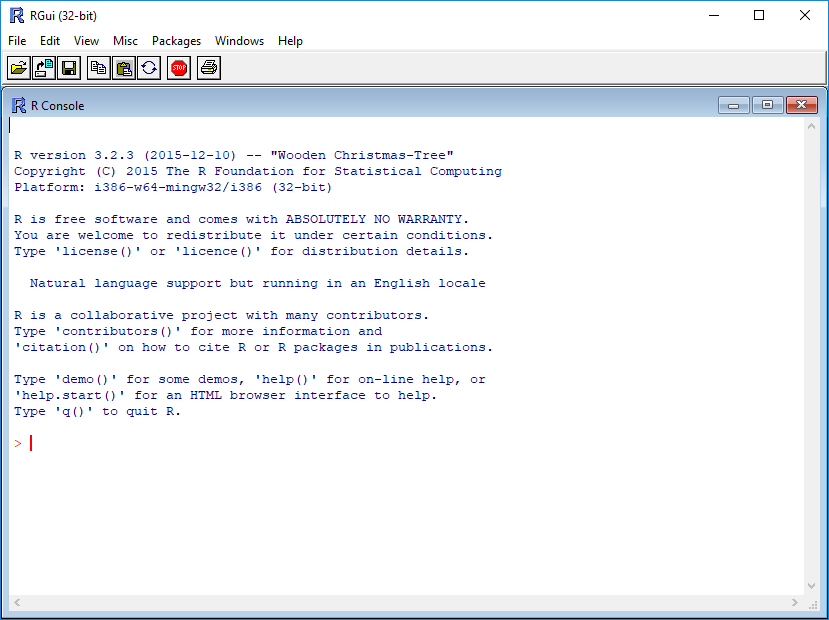
\includegraphics[width=2.76in,height=\textheight]{./images/console.png}

}

\end{figure}

While it is possible to work solely through the console or using a
command line interface, the ideal environment to work in R is RStudio.

\hypertarget{rstudio}{%
\subsection{RStudio}\label{rstudio}}

We will be working in
\href{https://www.rstudio.com/products/rstudio/download/}{RStudio}. The
easiest way to get started is to go to \href{https://posit.cloud/}{Posit
Cloud} and create a new project.

RStudio interface is conveniently organized into four divisions called
``panes''.

The Default Layout is:

\begin{itemize}
\tightlist
\item
  Top Left - \textbf{Source}: your scripts and documents
\item
  Bottom Left - \textbf{Console}: what R would look and be like without
  RStudio
\item
  Top Right - \textbf{Environment/History}: look here to see what you
  have done
\item
  Bottom Right - \textbf{Files} and more: see the contents of the
  project/working directory here, like your Script.R file
\end{itemize}

\begin{figure}

{\centering 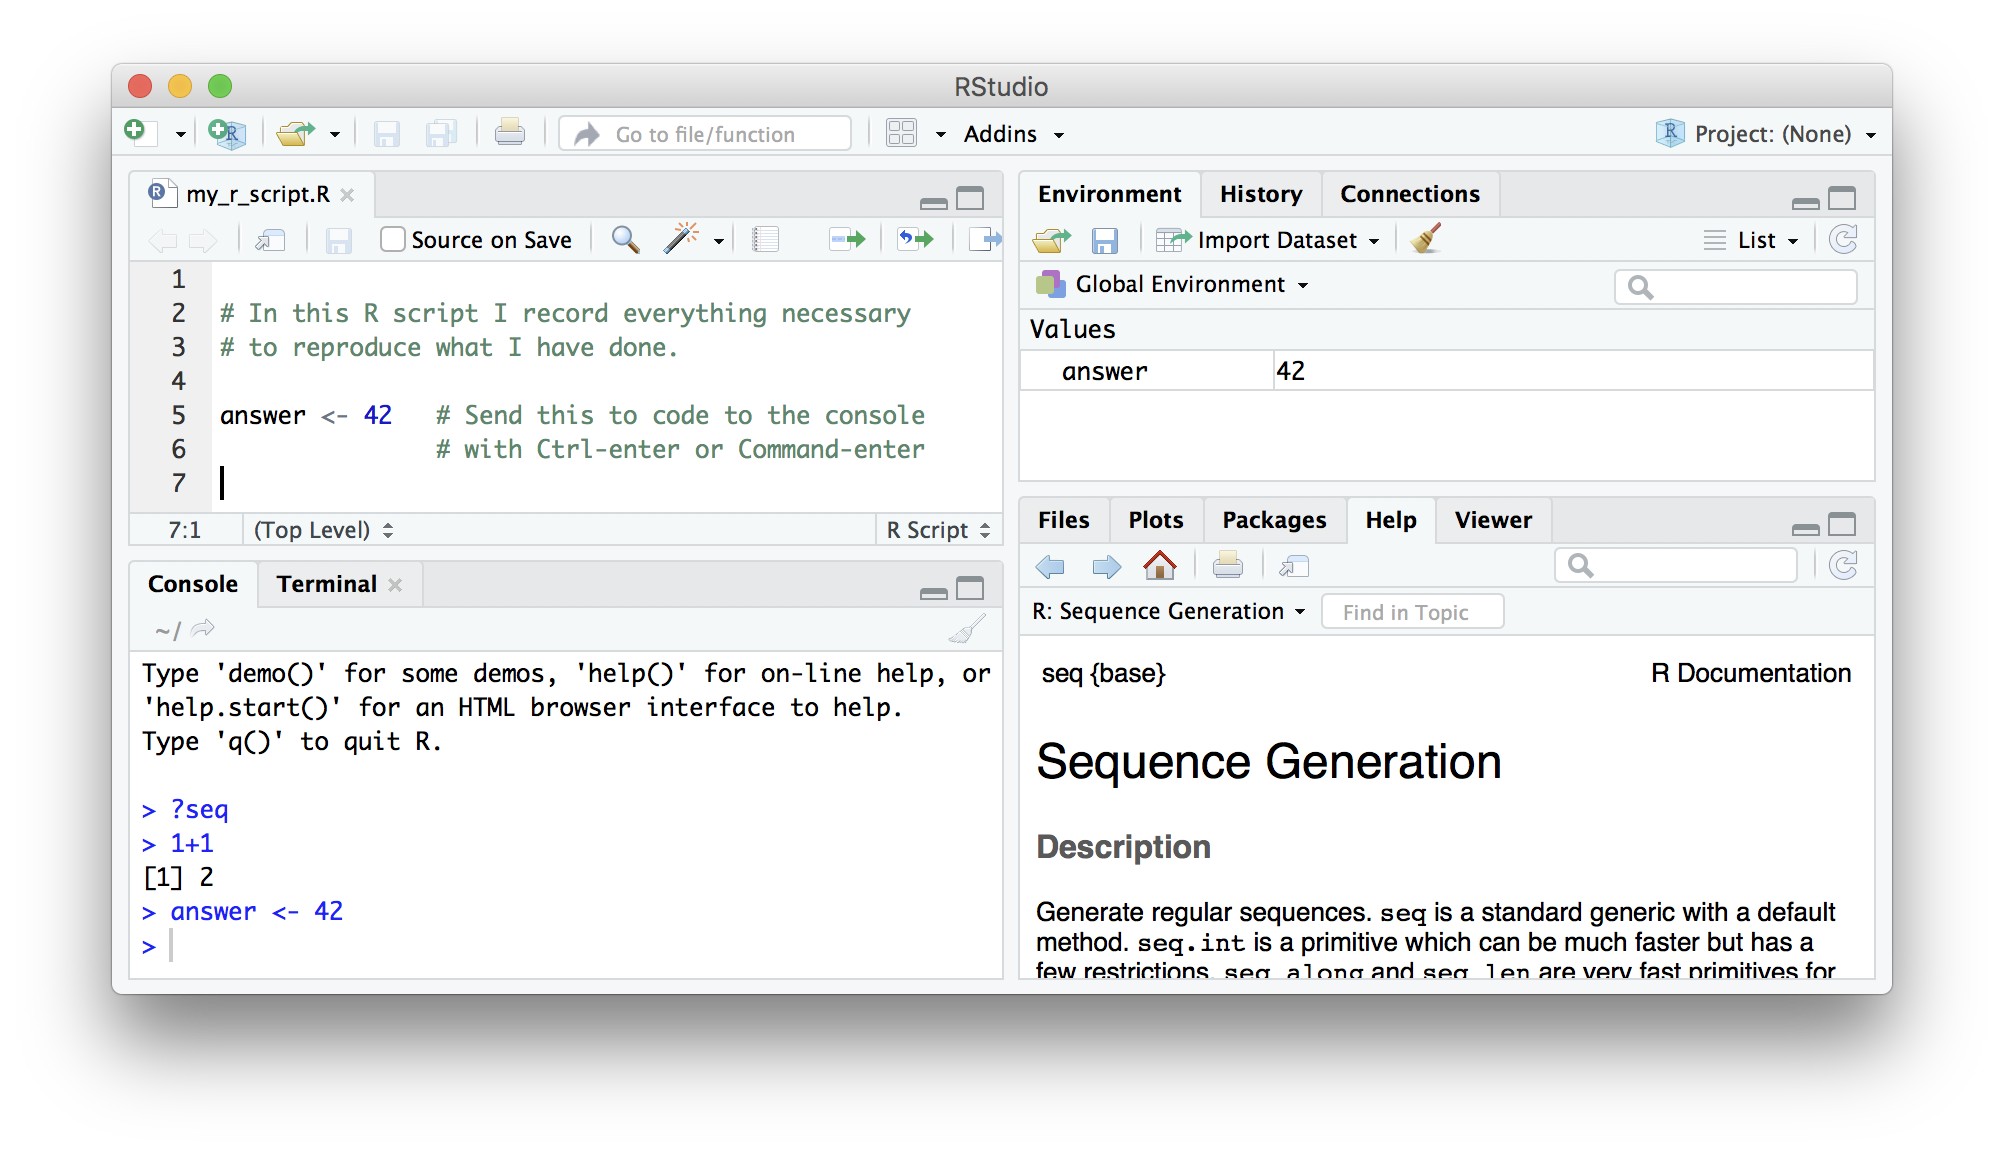
\includegraphics[width=6.68in,height=\textheight]{./images/rstudio.png}

}

\end{figure}

The placement of these panes and their content can be customized (see
menu, Tools -\textgreater{} Global Options -\textgreater{} Pane Layout)

\hypertarget{posit-cloud-formerly-rstudio-cloud}{%
\subsection{Posit Cloud (formerly RStudio
Cloud)}\label{posit-cloud-formerly-rstudio-cloud}}

Posit Cloud is a browser-based version of RStudio. It will allow you to
use RStudio without needing to download anything to your computer. You
can also easily share your R projects with others. To use Posit Cloud a
user account is required. While we recommend downloading RStudio for
routine R programming use, we will be using RStudio Cloud for this
training so we can easily share files and packages with you.

To access Posit Cloud proceed to \url{https://posit.cloud/} in a new
browser window or tab.

\hypertarget{using-this-book}{%
\section{Using this book}\label{using-this-book}}

\textbf{For these instructions code will appear in the gray box as
follows:}

\begin{verbatim}
fake code
\end{verbatim}

To run the code you can copy and paste the code and run it in your
RStudio session console at the prompt \texttt{\textgreater{}} which
looks like a greater than symbol.

\begin{verbatim}
> fake code
\end{verbatim}

The code can also be added to an R Script to be run.

When the code is run in RStudio the console prints out results like so:

\begin{verbatim}
[1] Result
\end{verbatim}

In this tutorial results from code will appear like so:

\begin{verbatim}
## [1] Result
\end{verbatim}

\hypertarget{working-in-the-console}{%
\section{Working in the Console}\label{working-in-the-console}}

The console is an interactive environment for RStudio, click on the
``Console'' pane, type \texttt{3\ +\ 3} and press enter. R displays the
result of the calculation.

\begin{Shaded}
\begin{Highlighting}[]
\DecValTok{3} \SpecialCharTok{+} \DecValTok{3}
\end{Highlighting}
\end{Shaded}

\begin{Shaded}
\begin{Highlighting}[]
\NormalTok{[1] 6}
\end{Highlighting}
\end{Shaded}

\texttt{+} is called an operator. R has the operators you would expect
for for basic mathematics:

\textbf{Arithmetic operators}

\begin{longtable}[]{@{}ll@{}}
\toprule()
operator & meaning \\
\midrule()
\endhead
+ & plus \\
- & minus \\
* & times \\
/ & divided by \\
\^{} & exponent \\
\bottomrule()
\end{longtable}

\textbf{Logical Operators}

\begin{longtable}[]{@{}ll@{}}
\toprule()
operator & meaning \\
\midrule()
\endhead
== & exactly equal \\
!= & not equal to \\
\textless{} & less than \\
\textless= & less than or equal to \\
\textgreater{} & greater than \\
\textgreater= & greater than or equal to \\
x\textbar y & x or y \\
x\&y & x and y \\
!x & not x \\
\bottomrule()
\end{longtable}

Spaces can be used to make code easier to read.

\begin{Shaded}
\begin{Highlighting}[]
\DecValTok{2} \SpecialCharTok{*} \DecValTok{2} \SpecialCharTok{==} \DecValTok{4}
\end{Highlighting}
\end{Shaded}

\begin{verbatim}
[1] TRUE
\end{verbatim}

You can also run commands in the consile for working with your computers
filesystem.

\begin{Shaded}
\begin{Highlighting}[]
\FunctionTok{getwd}\NormalTok{() }\CommentTok{\# similar to UNIX PWD}
\end{Highlighting}
\end{Shaded}

\hypertarget{working-in-the-terminal}{%
\section{Working in the Terminal}\label{working-in-the-terminal}}

The embedded Terminal in RStudio is a command-line interface within the
IDE, allowing users to execute system commands and interact with the
operating system directly. * It shares the same working directory as the
RStudio session and supports various commands for file management,
package installation, and more. * Integration into the IDE streamlines
workflows by eliminating the need to switch between applications,
enhancing productivity and enabling seamless interaction between R
programming and system administration tasks.

\begin{figure}

{\centering \includegraphics{https://i.imgur.com/4V0AR15.png}

}

\end{figure}

\bookmarksetup{startatroot}

\hypertarget{introduction}{%
\chapter{Introduction}\label{introduction}}

This is a book created from markdown and executable code.

See Knuth (1984) for additional discussion of literate programming.

\begin{Shaded}
\begin{Highlighting}[]
\DecValTok{1} \SpecialCharTok{+} \DecValTok{1}
\end{Highlighting}
\end{Shaded}

\begin{verbatim}
[1] 2
\end{verbatim}

\bookmarksetup{startatroot}

\hypertarget{summary}{%
\chapter{Summary}\label{summary}}

In summary, this book has no content whatsoever.

\begin{Shaded}
\begin{Highlighting}[]
\DecValTok{1} \SpecialCharTok{+} \DecValTok{1}
\end{Highlighting}
\end{Shaded}

\begin{verbatim}
[1] 2
\end{verbatim}

\bookmarksetup{startatroot}

\hypertarget{references}{%
\chapter*{References}\label{references}}
\addcontentsline{toc}{chapter}{References}

\markboth{References}{References}

\hypertarget{refs}{}
\begin{CSLReferences}{1}{0}
\leavevmode\vadjust pre{\hypertarget{ref-knuth84}{}}%
Knuth, Donald E. 1984. {``Literate Programming.''} \emph{Comput. J.} 27
(2): 97--111. \url{https://doi.org/10.1093/comjnl/27.2.97}.

\end{CSLReferences}



\end{document}
